\chapter{Indexação para Fingerprints}

\section{Introdução}

\begin{itemize}
    \item Matching local baseado em minúcias
    \begin{itemize}
        \item Abordagens antigas \cite{automated:hrechak1990,finger:willis2001}
        \item Associa cada minúcia as suas vizinhas em estruturas invariantes a rotação e distâncias\cite{globallocal:jiang2000,robustlocal:ratha2000}
        \item Baseada em cilindros, veja \cref{sec:mcc}
        \item Outros métodos que incluem mais características: local orientation field, local frequency, ridge shapes
    \end{itemize}
\end{itemize}

Estruturas locais de uma minúcia central podem ser baseadas em:
\begin{itemize}
    \item \textit{Vizinhos mais próximos}, que consideram as $k$ minúcias mais próximas \cite{globallocal:jiang2000}.
    
    A vantagem dessa representação é com relação ao tamanho fixo, facilitando no procedimento de comparação.
    
    \item \textit{Raio fixo}, que considera todas as minúcias dentro de um raio fixo, usada em \cite{robustlocal:ratha2000}.
    
    A vantagem dessa representação é a tolerância com relação a ruído (minúcias extras ou faltantes).
\end{itemize}

\section{Minutia Cylinder-Code}
\label{sec:mcc}

Baseada em \cite{mccmatching:cappelli2010,mccindexing:cappelli2010}

\subsection{Representação}

Uma representação tridimensional de minúcias baseada em distâncias entre minúcias e ângulos relativos. A representação recebe o nome de Minutia Cylinder-Code (MCC) e tem como características principais: invariância de rotação, tamanho fixo e orientada a codificação binária.

O esquema de representação é um cilindro segmentado, como na \cref{fig:mcc}. O cilindro é um recorte de um cubo dividido em células, onde cada uma possui um valor indexado por $C_m[i, j, k]$.

\begin{figure}
    \centering
    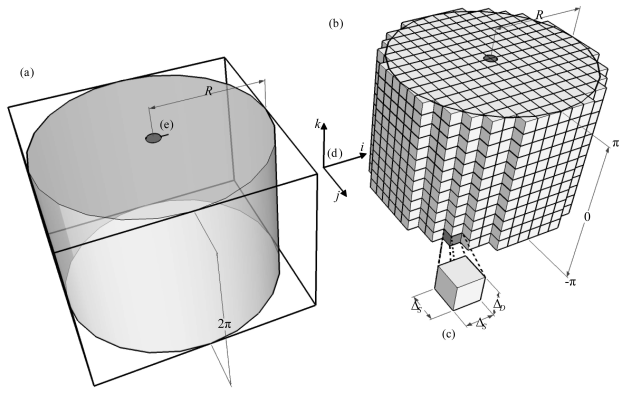
\includegraphics[width=0.6\textwidth]{imgs/fingerprint_cylinder_code.png}
    \caption{Representação de um MCC.}
    \label{fig:mcc}
\end{figure}

O cálculo dos valores de $C_m[i, j, k]$ é complicado, mas essencialmente envolve as seguintes ideias:
\begin{itemize}
\item Verifica se está em uma região válida: dentro do cilindro e dentro do \textit{convex hull} da fingerprint.
\item Calcula a contribuição de cada minúcia vizinha usando uma Gaussiana, \cref{fig:mccdist}.
\item Calcula a contribuição de cada minúcia usando a diferença entre a orientação.
\end{itemize}

\begin{figure}
    \centering
    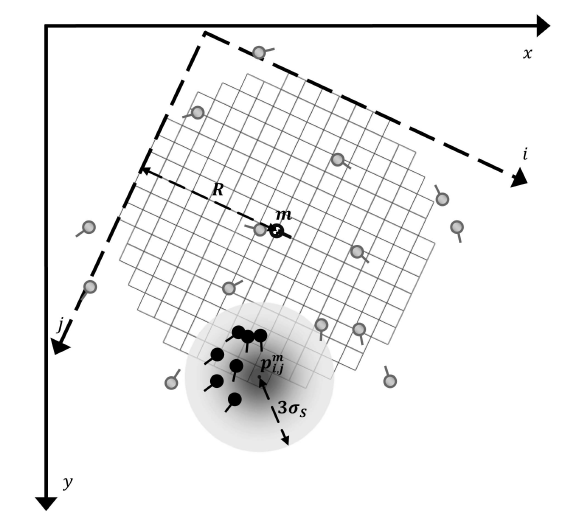
\includegraphics[width=0.6\textwidth]{imgs/eval_cylinder.png}
    \caption{Contribuição da distância de uma minúcia vizinha. Cores mais escuras refletem uma maior contribuição.}
    \label{fig:mccdist}
\end{figure}

\subsection{Similaridade}

A similaridade entre dois cilindros é obtida a partir do seguinte procedimento:
\begin{enumerate}
    \item Lineariza o cilindro em um vetor, similar a operação de \texttt{reshape}. Por exemplo, o cilindro de uma minúcia $a$, $C_a[i, j, k]$, é linearizado em $\mathbf{c}_a$.
    \item Seleciona todas as entradas comparáveis desses vetores (células que são \textit{válidas} em ambos) que dão origem aos vetores $\tilde{\mathbf{v}}_a$ e $\tilde{\mathbf{v}}_b$.
    \item Na implementação binária, é realizado um XOR bit a bit entre os vetores.
    \begin{equation}
        \gamma(\tilde{\mathbf{v}}_a, \tilde{\mathbf{v}}_b) =
            1 - \frac{\|\tilde{\mathbf{v}}_a \oplus \tilde{\mathbf{v}}_b\|}{\|\tilde{\mathbf{v}}_a\| + \|\tilde{\mathbf{v}}_b\|}
    \end{equation}
\end{enumerate}

\subsection{Indexação}

Para a indexação de um MCC é empregado um esquema de \textit{locality-sensitive hashing} (LSH), \cite{lsh:gionis1999,approximate:indyk1998}.

O procedimento consiste em:
\begin{enumerate}
    \item Seja $\mathbf{v}_m$ o vetor obtido da linearização de um cilindro.
    \item É feita a projeção de $\mathbf{v}_m$ em um subespaço $\mathbf{h}_m$. A projeção é obtida simplesmente ao escolher um subconjunto dos índices $H$ do vetor original.
    \begin{equation}
        \mathbf{h}_m = \mathbf{v}_m[H]
    \end{equation}
    \item O conjunto $H$ define uma função que mapeia um vetor binário $\mathbf{v}_m$ em um número natural obtido ao interpretar o vetor binário $\mathbf{h}_m$ como um número natural.
    \begin{equation}
        h_H: \{0, 1\}^n \rightarrow \mathbb{N}
    \end{equation}
    \item São definidos $\ell$ conjuntos $H_1, H_2, \ldots, H_\ell$, cada um com uma função $h_{H_i}$.
    \item O índice por sua vez é um conjunto de \textit{hash tables}, $\mathbb{H}_1, \mathbb{H}_2, \ldots, \mathbb{H}_\ell$, onde cada hash table tem os seus buckets definidos pela função $h_{H_i}$.
    \item A indexação segue fazendo a consulta do vetor desejado em cada hash table, retornando os candidatos.
    \item Por fim, os candidatos são ranqueados usando a \textit{distância de Hamming} entre os vetores.
\end{enumerate}

O procedimento enumerado acima é ilustrado na \cref{fig:lshmcc}.

\begin{figure}
    \centering
    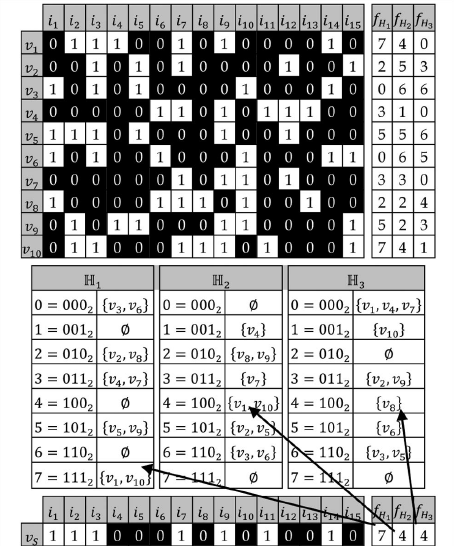
\includegraphics[width=0.8\textwidth]{imgs/cylinder_lsh.png}
    \caption{Ilustração do procedimento de indexação usando LSH de um MCC.}
    \label{fig:lshmcc}
\end{figure}

\printbibliography